\documentclass[12pt, a4paper]{article}

% ──────────────────────────────────────
% Packages
% ──────────────────────────────────────
\usepackage[utf8]{inputenc}
\usepackage[T1]{fontenc}
\usepackage{lmodern}
\usepackage[margin=1in]{geometry}
\usepackage{graphicx}
\usepackage{amsmath, amssymb}
\usepackage{booktabs}
\usepackage{hyperref}
\usepackage{caption}
\usepackage{subcaption}
\usepackage{float}
\usepackage{enumitem}
\usepackage{xcolor}
\usepackage{listings}
\usepackage{fancyhdr}
\usepackage{titlesec}


% ──────────────────────────────────────
% Styling
% ──────────────────────────────────────
\hypersetup{
    colorlinks=true,
    linkcolor=blue!70!black,
    citecolor=green!50!black,
    urlcolor=blue!60!black
}

\pagestyle{fancy}
\fancyhf{}
\fancyhead[L]{\small ExamWise --- Milestone~1}
\fancyhead[R]{\small EPOCH PIONEERS}
\fancyfoot[C]{\thepage}
\renewcommand{\headrulewidth}{0.4pt}

\lstset{
    basicstyle=\ttfamily\small,
    keywordstyle=\color{blue!70!black}\bfseries,
    commentstyle=\color{green!50!black}\itshape,
    stringstyle=\color{red!60!black},
    backgroundcolor=\color{gray!5},
    frame=single,
    rulecolor=\color{gray!40},
    breaklines=true,
    captionpos=b,
    numbers=left,
    numberstyle=\tiny\color{gray},
    tabsize=4
}

% ──────────────────────────────────────
% Title
% ──────────────────────────────────────
\title{
    \vspace{-1cm}
    \textbf{\Large ExamWise: Intelligent Exam Question\\
    Difficulty Analysis System}\\[0.5em]
    \large Milestone~1 --- Difficulty Analysis \& Baseline System Setup\\[0.3em]
    \normalsize Project Report
}

\author{
    \textbf{Team EPOCH PIONEERS}\\[0.5em]
    \begin{tabular}{c}
        Department of Computer Science and Engineering
    \end{tabular}
}

\date{\today}

% ══════════════════════════════════════
\begin{document}
% ══════════════════════════════════════

\maketitle
\thispagestyle{fancy}

% ──────────────────────────────────────
\begin{abstract}
Traditional examination evaluation methods determine question difficulty only after students have attempted the exam, limiting the ability of educators to design balanced assessments in advance. This project presents \textbf{ExamWise}, a machine learning--based system that analyzes exam-style questions and predicts their difficulty level (\textit{Easy}, \textit{Medium}, \textit{Hard}) using textual features derived from natural language processing techniques. In Milestone~1, we establish the complete data pipeline---from raw Stack Overflow question--answer data to a trained Logistic Regression classifier---achieving an overall accuracy of $65.71\%$. We also build analytical visualizations and a Streamlit-based web interface for interactive exploration. This report documents the methodology, implementation, results, and future directions of the project.
\end{abstract}

\tableofcontents
\newpage

% ══════════════════════════════════════
\section{Introduction}
\label{sec:intro}
% ══════════════════════════════════════

In conventional educational assessment, question difficulty is understood only retrospectively---after students take the exam and scores are aggregated~\cite{lord1980applications}. This reactive paradigm limits instructors who wish to construct well-balanced question papers \emph{before} administration.

\textbf{ExamWise} addresses this gap by building a predictive system that estimates question difficulty from the question text itself, without requiring prior student performance data. The system leverages supervised machine learning and natural language processing (NLP) to classify questions into three difficulty tiers.

\subsection{Problem Statement}
Given a corpus of questions with associated community response behaviour, the objective is to:
\begin{enumerate}[noitemsep]
    \item Derive difficulty labels from historical engagement metrics.
    \item Train a text-based classifier that generalises to unseen questions.
    \item Provide analytical dashboards for question-level insights.
\end{enumerate}

\subsection{Scope of Milestone~1}
Milestone~1 delivers the foundational components:
\begin{itemize}[noitemsep]
    \item Data acquisition, reduction, and labelling pipeline.
    \item Feature extraction using Bag-of-Words vectorisation.
    \item Baseline Logistic Regression model for multi-class classification.
    \item Analytical visualisations (difficulty distribution, accuracy analysis, hardest questions).
    \item Streamlit web application for end-to-end interaction.
\end{itemize}

% ══════════════════════════════════════
\section{Literature Review}
\label{sec:litreview}
% ══════════════════════════════════════

Automated question difficulty estimation has been explored through several approaches in educational data mining:

\begin{itemize}
    \item \textbf{Item Response Theory (IRT):} Classical psychometric models estimate item difficulty as a latent parameter from response patterns~\cite{hambleton1991fundamentals}. However, IRT requires observed response data and cannot predict difficulty for new items.
    
    \item \textbf{Text-based approaches:} Recent work uses NLP features (readability scores, syntactic complexity, word frequency) to predict difficulty from question text alone~\cite{ha2019automated}. TF--IDF and word embeddings are commonly used representations.
    
    \item \textbf{Community Q\&A platforms:} Stack Overflow data has been used as a proxy for educational content, where answer scores and response rates serve as engagement-based difficulty indicators~\cite{anderson2012discovering}.
\end{itemize}

Our approach combines community engagement metrics for label derivation with text-based features for classification, enabling prediction on unseen questions.

% ══════════════════════════════════════
\section{Dataset}
\label{sec:dataset}
% ══════════════════════════════════════

\subsection{Data Source}
We use the \textbf{StackSample} dataset from Kaggle~\cite{stacksample}, which contains a 10\% sample of Stack Overflow questions and answers. The raw dataset comprises:

\begin{table}[H]
\centering
\caption{Raw dataset statistics}
\label{tab:raw-data}
\begin{tabular}{lrr}
\toprule
\textbf{File} & \textbf{Original Rows} & \textbf{Reduced Rows} \\
\midrule
\texttt{Questions.csv} & $\sim$19.9M & 15{,}000 \\
\texttt{Answers.csv}   & $\sim$17.7M & 15{,}000 \\
\texttt{Tags.csv}      & $\sim$1.9M  & 15{,}000 \\
\bottomrule
\end{tabular}
\end{table}

\subsection{Data Reduction}
Due to computational constraints, the dataset is reduced to 15{,}000 rows per file using \texttt{data\_reduction.py}. The reduction preserves referential integrity by:
\begin{enumerate}[noitemsep]
    \item Selecting the first 15{,}000 questions.
    \item Filtering answers whose \texttt{ParentId} matches the selected question IDs.
    \item Filtering tags corresponding to those question IDs.
\end{enumerate}

\subsection{Difficulty Labelling}
Since real student response data is unavailable, we use community engagement as a proxy. The \textbf{difficulty score} for each question is computed as:

\begin{equation}
    \text{difficulty\_score} = 1 - \frac{\text{max\_answer\_score}}{\text{max\_answer\_score} + \text{answer\_count} + 1}
    \label{eq:difficulty}
\end{equation}

The intuition is that questions with high-scoring answers relative to their answer count are ``easier'' (the community converged on a good solution), while questions with low-scoring or few answers are ``harder''.

After min--max normalisation to $[0,1]$, labels are assigned using fixed thresholds:

\begin{equation}
    \text{label} =
    \begin{cases}
        \textit{Easy}   & \text{if } \text{difficulty\_score} < 0.33 \\
        \textit{Medium} & \text{if } 0.33 \leq \text{difficulty\_score} < 0.66 \\
        \textit{Hard}   & \text{if } \text{difficulty\_score} \geq 0.66
    \end{cases}
    \label{eq:thresholds}
\end{equation}

\subsection{Label Distribution}
The resulting distribution is highly imbalanced (Table~\ref{tab:label-dist}):

\begin{table}[H]
\centering
\caption{Difficulty label distribution in the processed dataset}
\label{tab:label-dist}
\begin{tabular}{lrr}
\toprule
\textbf{Label} & \textbf{Count} & \textbf{Percentage} \\
\midrule
Hard   & 11{,}280 & 75.2\% \\
Medium &  2{,}192 & 14.6\% \\
Easy   &  1{,}528 & 10.2\% \\
\midrule
\textbf{Total} & \textbf{15{,}000} & \textbf{100\%} \\
\bottomrule
\end{tabular}
\end{table}

% ══════════════════════════════════════
\section{Methodology}
\label{sec:methodology}
% ══════════════════════════════════════

Figure~\ref{fig:pipeline} illustrates the end-to-end pipeline.

\begin{figure}[H]
\centering
\fbox{\parbox{0.85\textwidth}{\centering
\texttt{Raw CSVs} $\;\xrightarrow{\text{Reduce}}\;$ \texttt{15k subset} $\;\xrightarrow{\text{Feature Eng.}}\;$ \texttt{Labelled Data}\\[0.5em]
$\;\xrightarrow{\text{Preprocess}}\;$ \texttt{Clean Text} $\;\xrightarrow{\text{Vectorise}}\;$ \texttt{BoW Matrix} $\;\xrightarrow{\text{Train}}\;$ \texttt{LR Model}\\[0.5em]
$\;\xrightarrow{\text{Evaluate}}\;$ \texttt{Metrics} $\;\xrightarrow{\text{Visualise}}\;$ \texttt{Dashboard}
}}
\caption{ExamWise Milestone~1 processing pipeline}
\label{fig:pipeline}
\end{figure}

\subsection{Feature Engineering}
For each question, the following features are computed from the answer data:

\begin{table}[H]
\centering
\caption{Engineered features per question}
\label{tab:features}
\begin{tabular}{ll}
\toprule
\textbf{Feature} & \textbf{Description} \\
\midrule
\texttt{max\_answer\_score}       & Highest score among all answers \\
\texttt{avg\_answer\_score}       & Mean score across all answers \\
\texttt{answer\_score\_variance}  & Variance of answer scores \\
\texttt{answer\_count}            & Number of answers received \\
\texttt{question\_score}          & Community score of the question \\
\texttt{ratio}                    & $\frac{\text{max\_answer\_score}}{\text{answer\_count} + 1}$ \\
\bottomrule
\end{tabular}
\end{table}

\subsection{Text Preprocessing}
The question body undergoes the following transformations:
\begin{enumerate}[noitemsep]
    \item \textbf{HTML stripping:} Removal of HTML tags using regex \texttt{\textless{}[\^{}\textgreater{}]*\textgreater{}}.
    \item \textbf{Non-alphabetic removal:} Retains only alphabetical characters.
    \item \textbf{Lowercasing:} Uniform case normalisation.
    \item \textbf{Stop word removal:} English stop words excluded during vectorisation.
\end{enumerate}

\subsection{Text Vectorisation}
The cleaned text is transformed into a numerical feature matrix using \texttt{CountVectorizer} (Bag-of-Words) from scikit-learn~\cite{sklearn}, with English stop words removed. Each question is represented as a sparse vector of word counts.

\subsection{Classification Model}
A \textbf{Logistic Regression} classifier is trained on the vectorised text features for multi-class difficulty prediction. The model uses the one-vs-rest (OvR) scheme:

\begin{equation}
    P(y = k \mid \mathbf{x}) = \frac{e^{\mathbf{w}_k^\top \mathbf{x} + b_k}}{\sum_{j=1}^{K} e^{\mathbf{w}_j^\top \mathbf{x} + b_j}}
    \label{eq:softmax}
\end{equation}

where $\mathbf{x}$ is the BoW feature vector, $\mathbf{w}_k$ and $b_k$ are the weight and bias for class $k$, and $K = 3$ (Easy, Medium, Hard).

\subsection{Train--Test Split}
The dataset is split into 70\% training and 30\% testing:
\begin{itemize}[noitemsep]
    \item Training set: 10{,}500 samples
    \item Test set: 4{,}500 samples
\end{itemize}

% ══════════════════════════════════════
\section{Results}
\label{sec:results}
% ══════════════════════════════════════

\subsection{Model Performance}

\begin{table}[H]
\centering
\caption{Classification report on the test set ($n = 4{,}500$)}
\label{tab:metrics}
\begin{tabular}{lcccc}
\toprule
\textbf{Class} & \textbf{Precision} & \textbf{Recall} & \textbf{F1-Score} & \textbf{Support} \\
\midrule
Easy   & 0.14 & 0.10 & 0.12 & 473  \\
Medium & 0.20 & 0.15 & 0.17 & 643  \\
Hard   & 0.76 & 0.83 & 0.80 & 3{,}384 \\
\midrule
\textbf{Accuracy}     & \multicolumn{4}{c}{$\mathbf{0.6571}$ (65.71\%)} \\
\textbf{Macro Avg}    & 0.37 & 0.36 & 0.36 & 4{,}500 \\
\textbf{Weighted Avg} & 0.62 & 0.66 & 0.64 & 4{,}500 \\
\bottomrule
\end{tabular}
\end{table}

\textbf{Key observations:}
\begin{itemize}[noitemsep]
    \item The model achieves $65.71\%$ overall accuracy, driven largely by correct predictions on the majority class (\textit{Hard}).
    \item The \textit{Easy} class has an F1-score of only $0.12$, indicating the model struggles severely with minority classes.
    \item The macro-averaged F1 of $0.36$ reveals that per-class performance is not balanced.
    \item The class imbalance (75\% \textit{Hard}) is the primary cause of poor minority-class performance.
\end{itemize}

\subsection{Visualisations}

\begin{figure}[H]
    \centering
    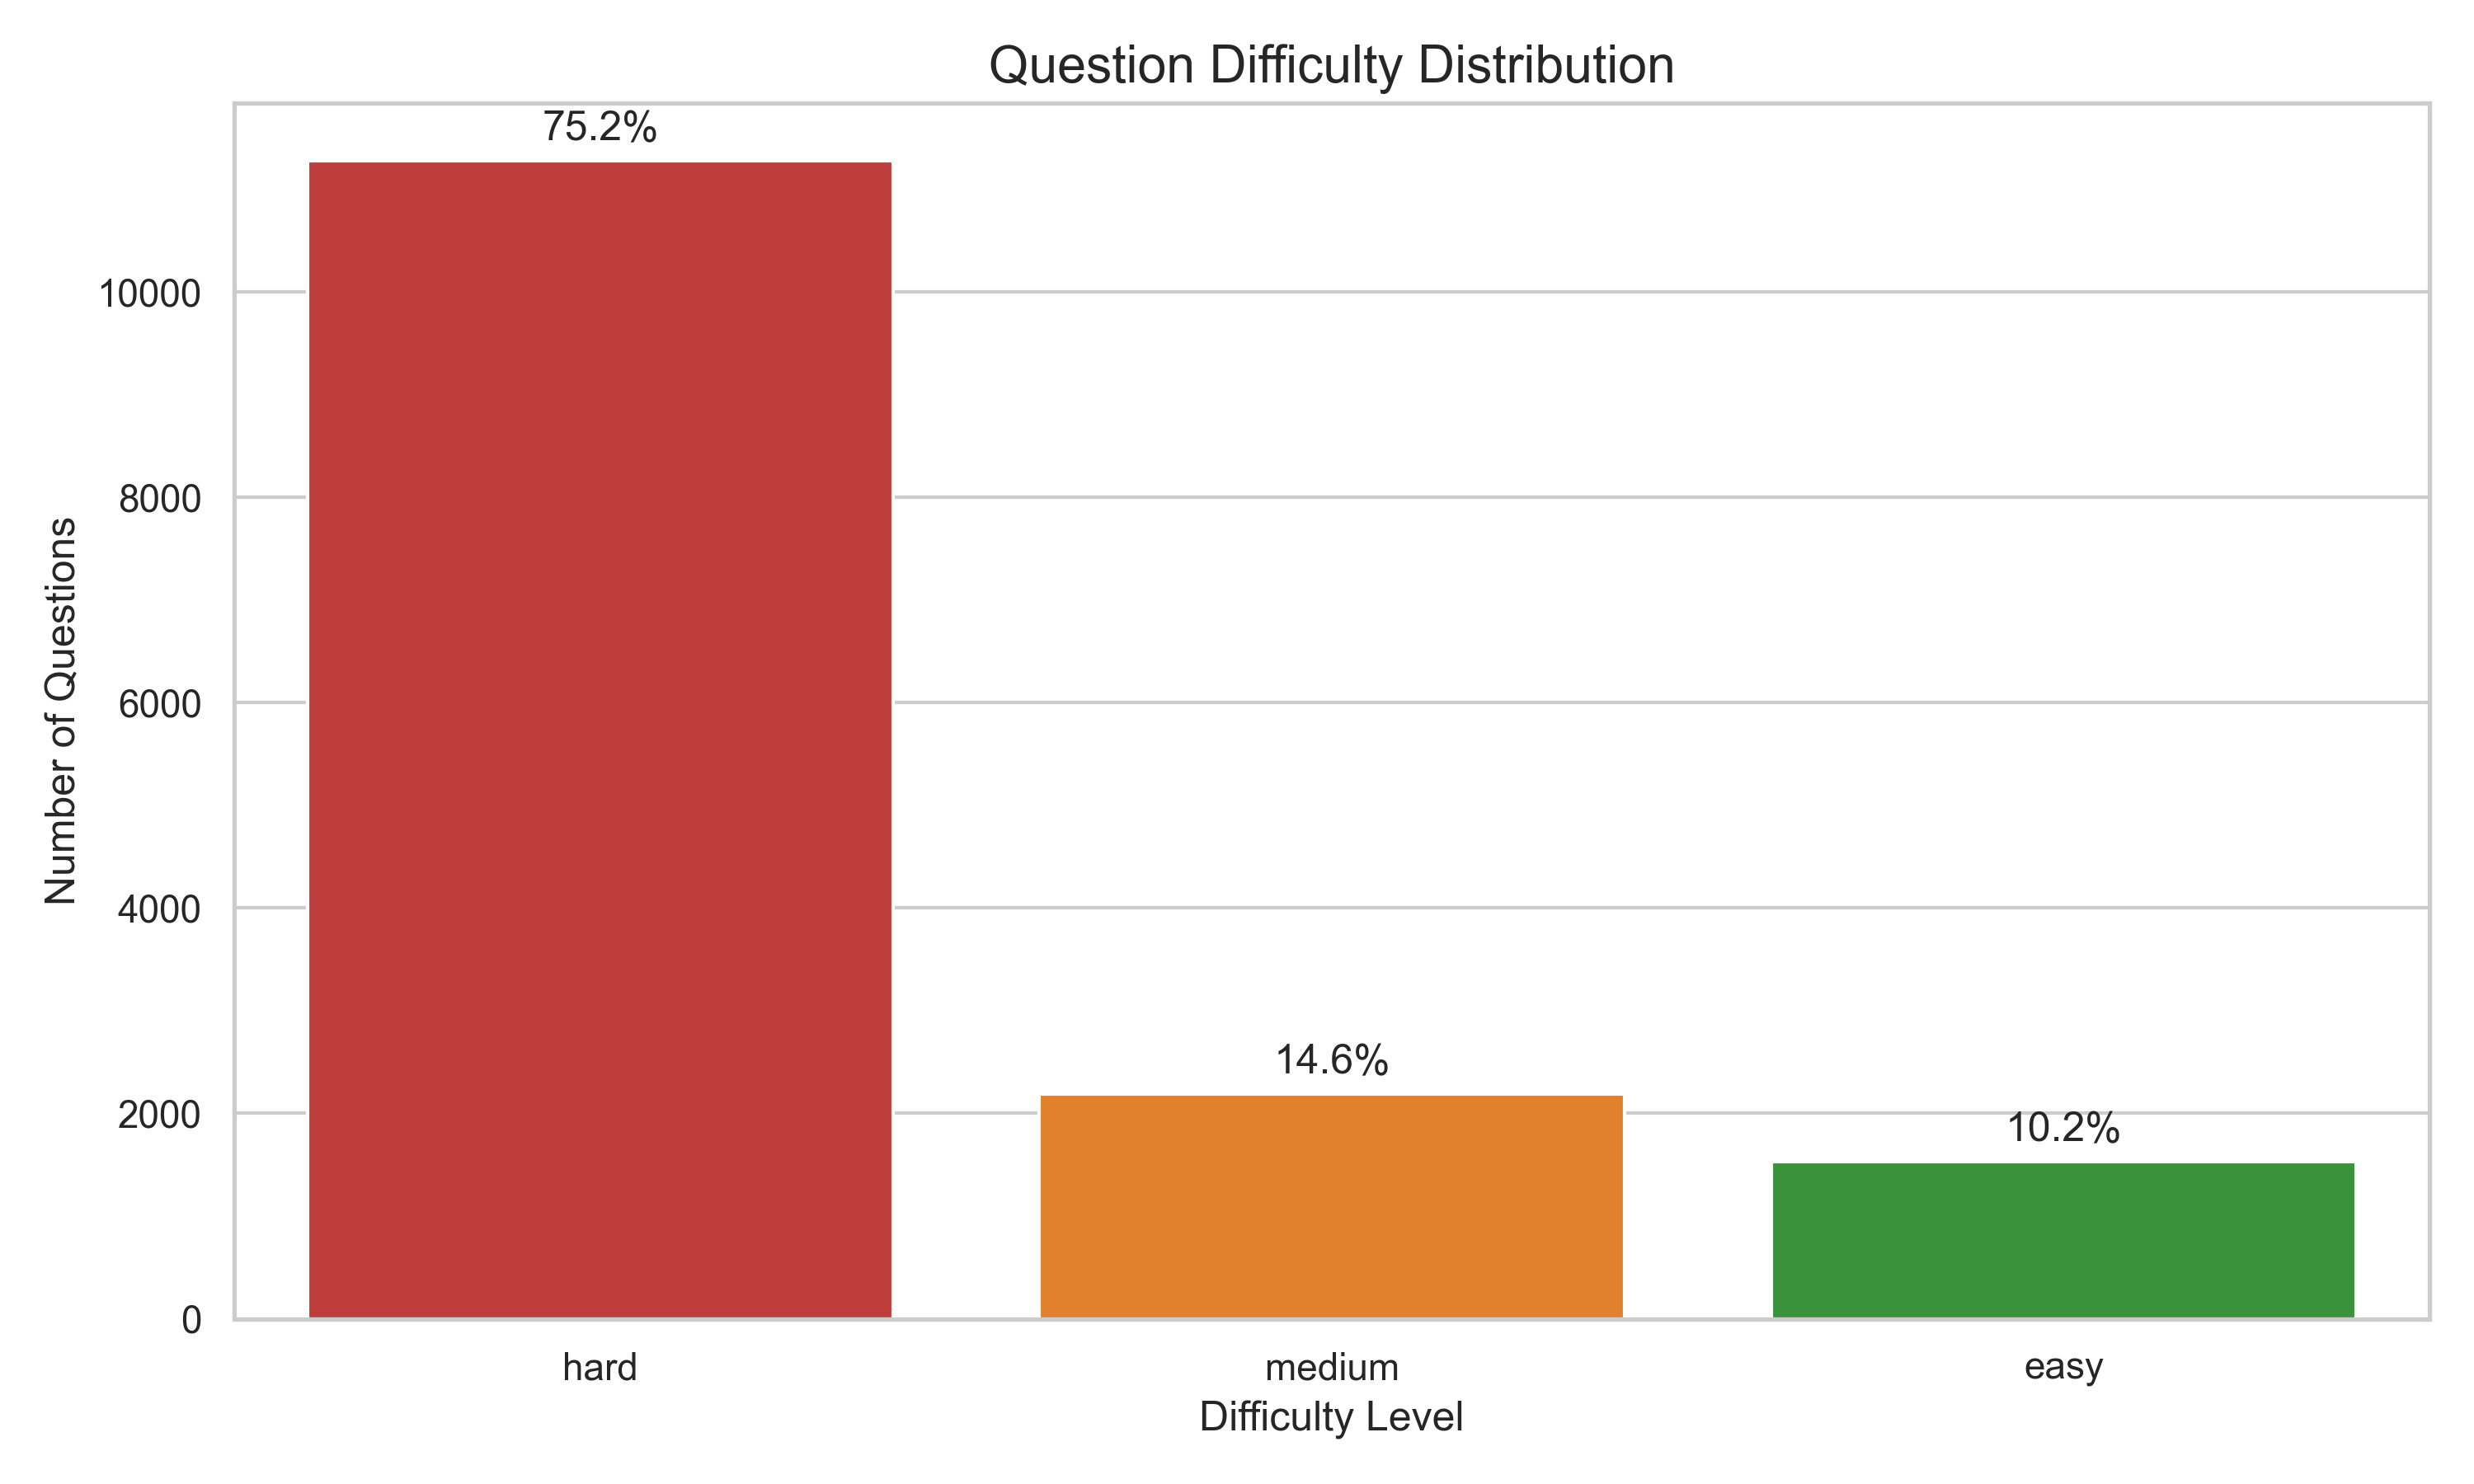
\includegraphics[width=0.8\textwidth]{figures/difficulty_distribution.png}
    \caption{Distribution of difficulty labels across the processed dataset. The dataset is heavily skewed towards \textit{Hard} questions (75.2\%).}
    \label{fig:diff-dist}
\end{figure}

\begin{figure}[H]
    \centering
    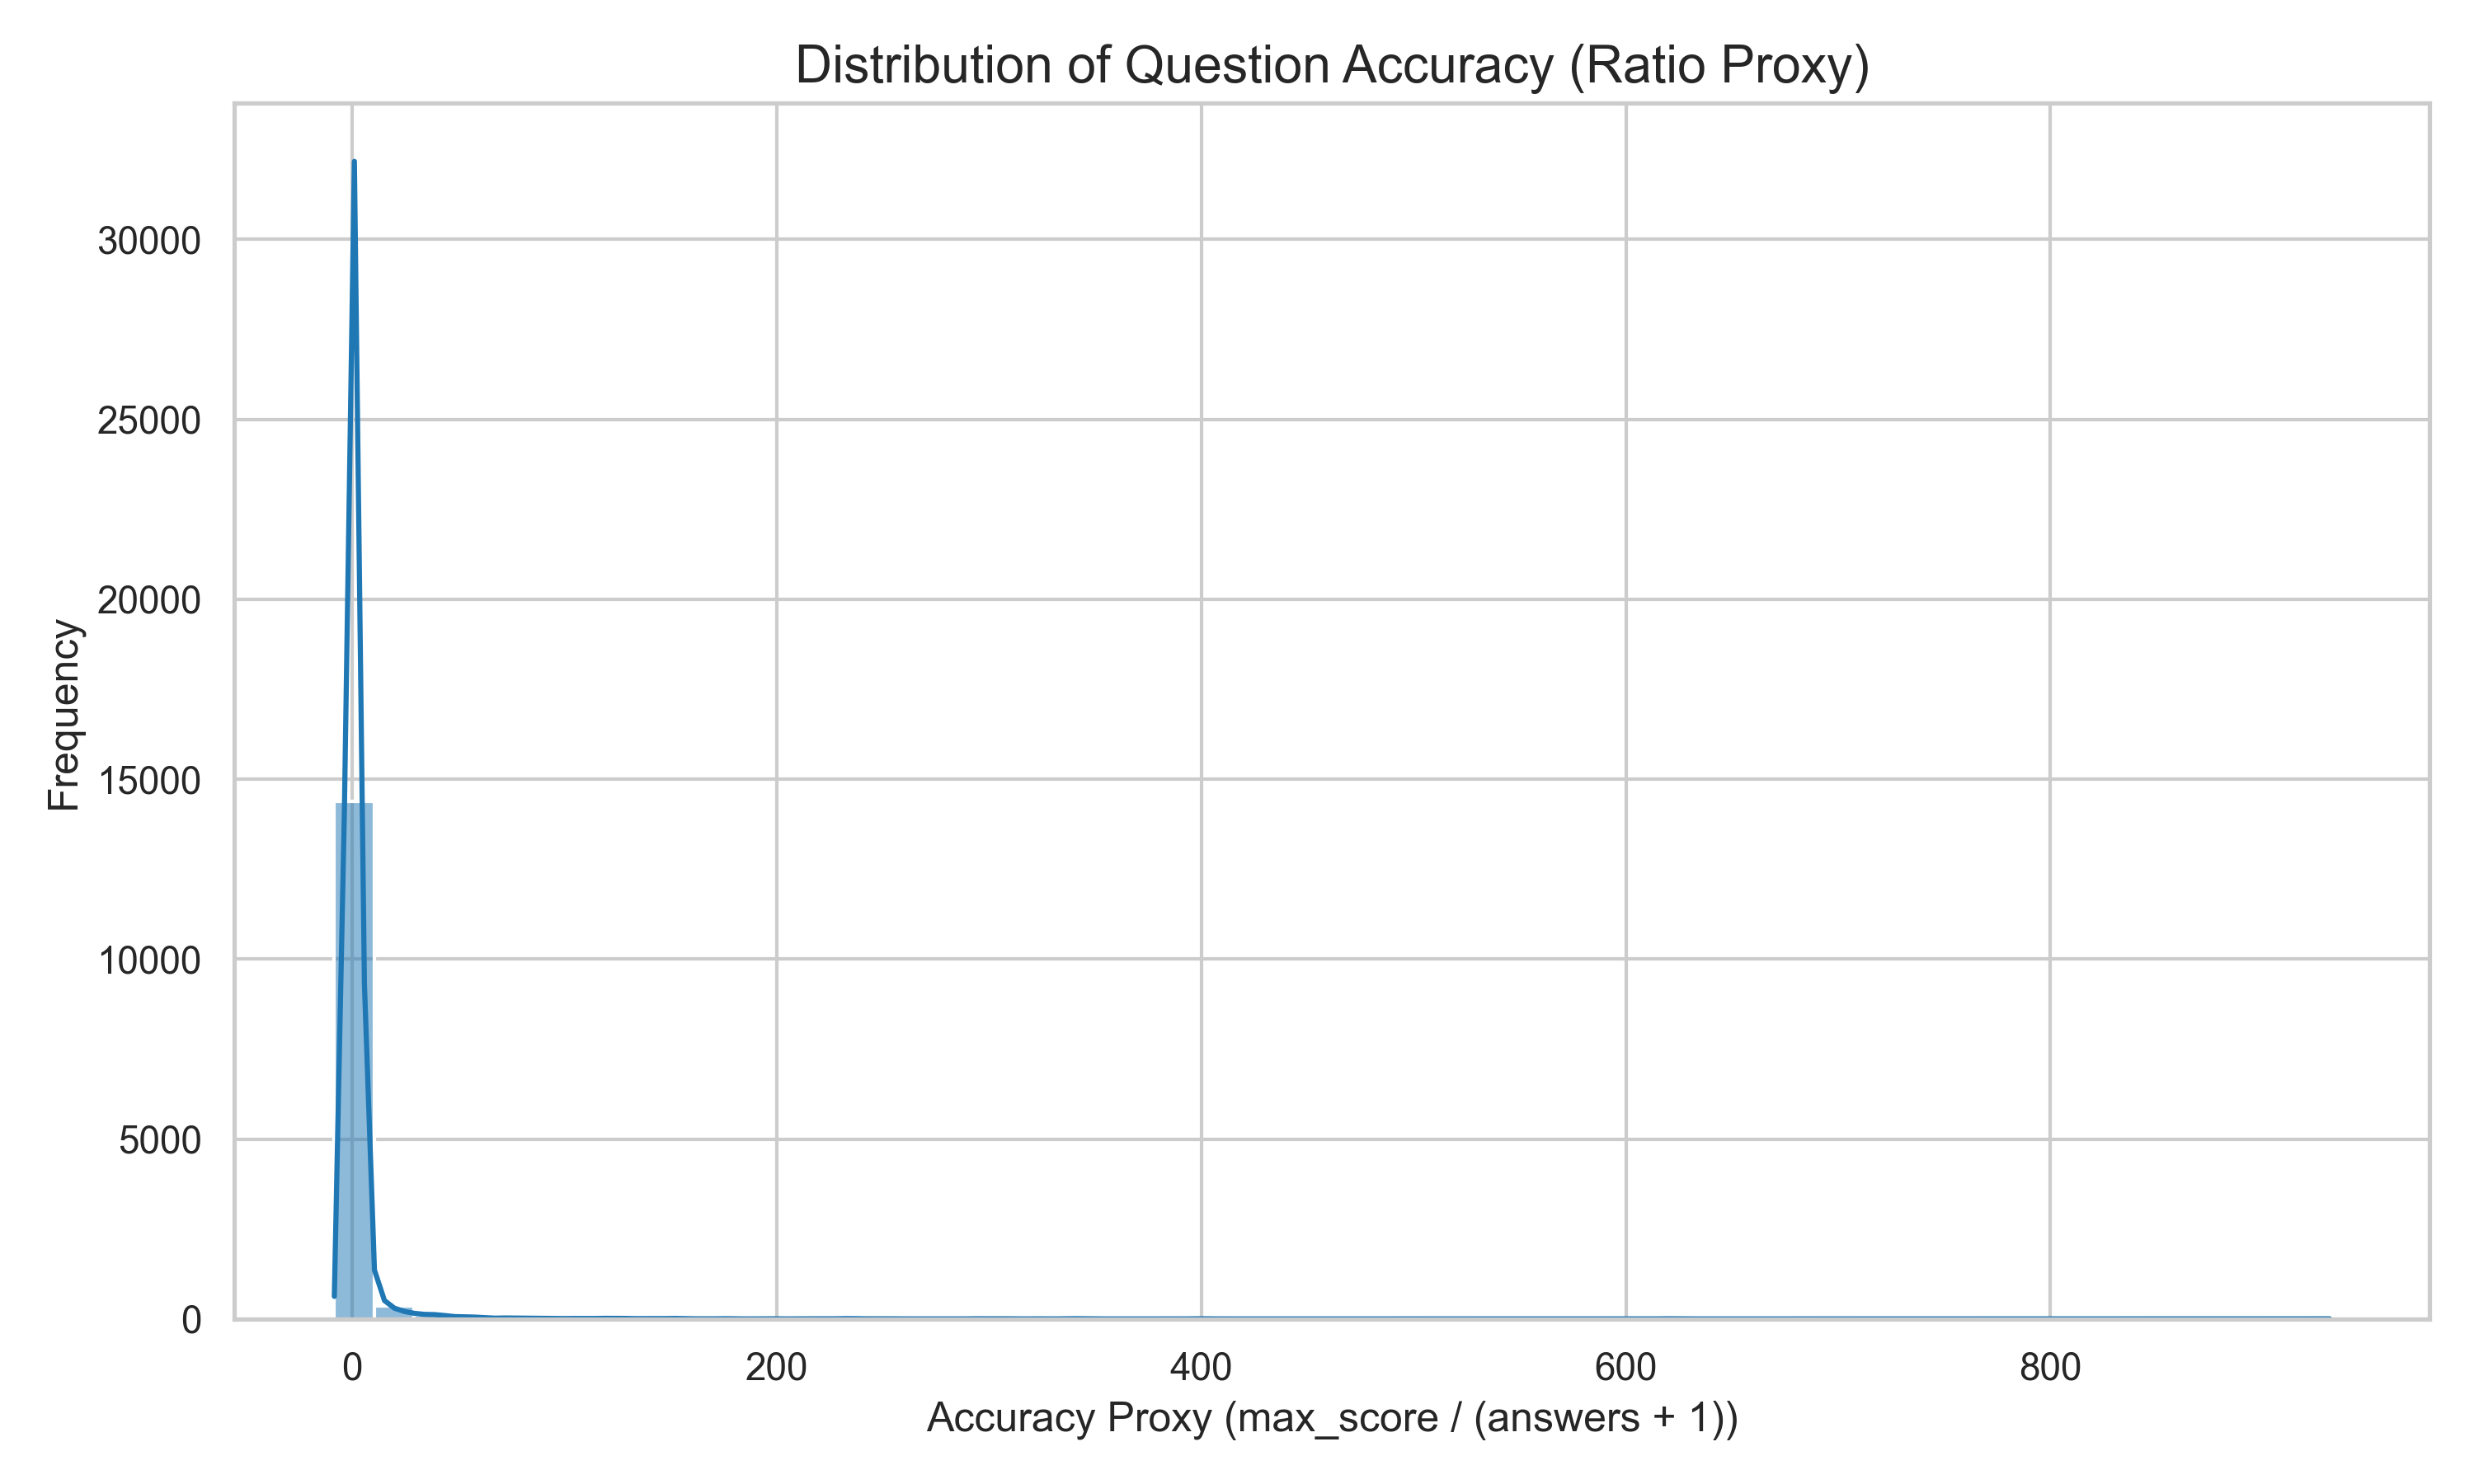
\includegraphics[width=0.8\textwidth]{figures/accuracy_distribution.png}
    \caption{Distribution of the accuracy proxy metric ($\text{ratio} = \frac{\text{max\_answer\_score}}{\text{answer\_count} + 1}$). The distribution is right-skewed, with most questions concentrated near zero.}
    \label{fig:acc-dist}
\end{figure}

\begin{figure}[H]
    \centering
    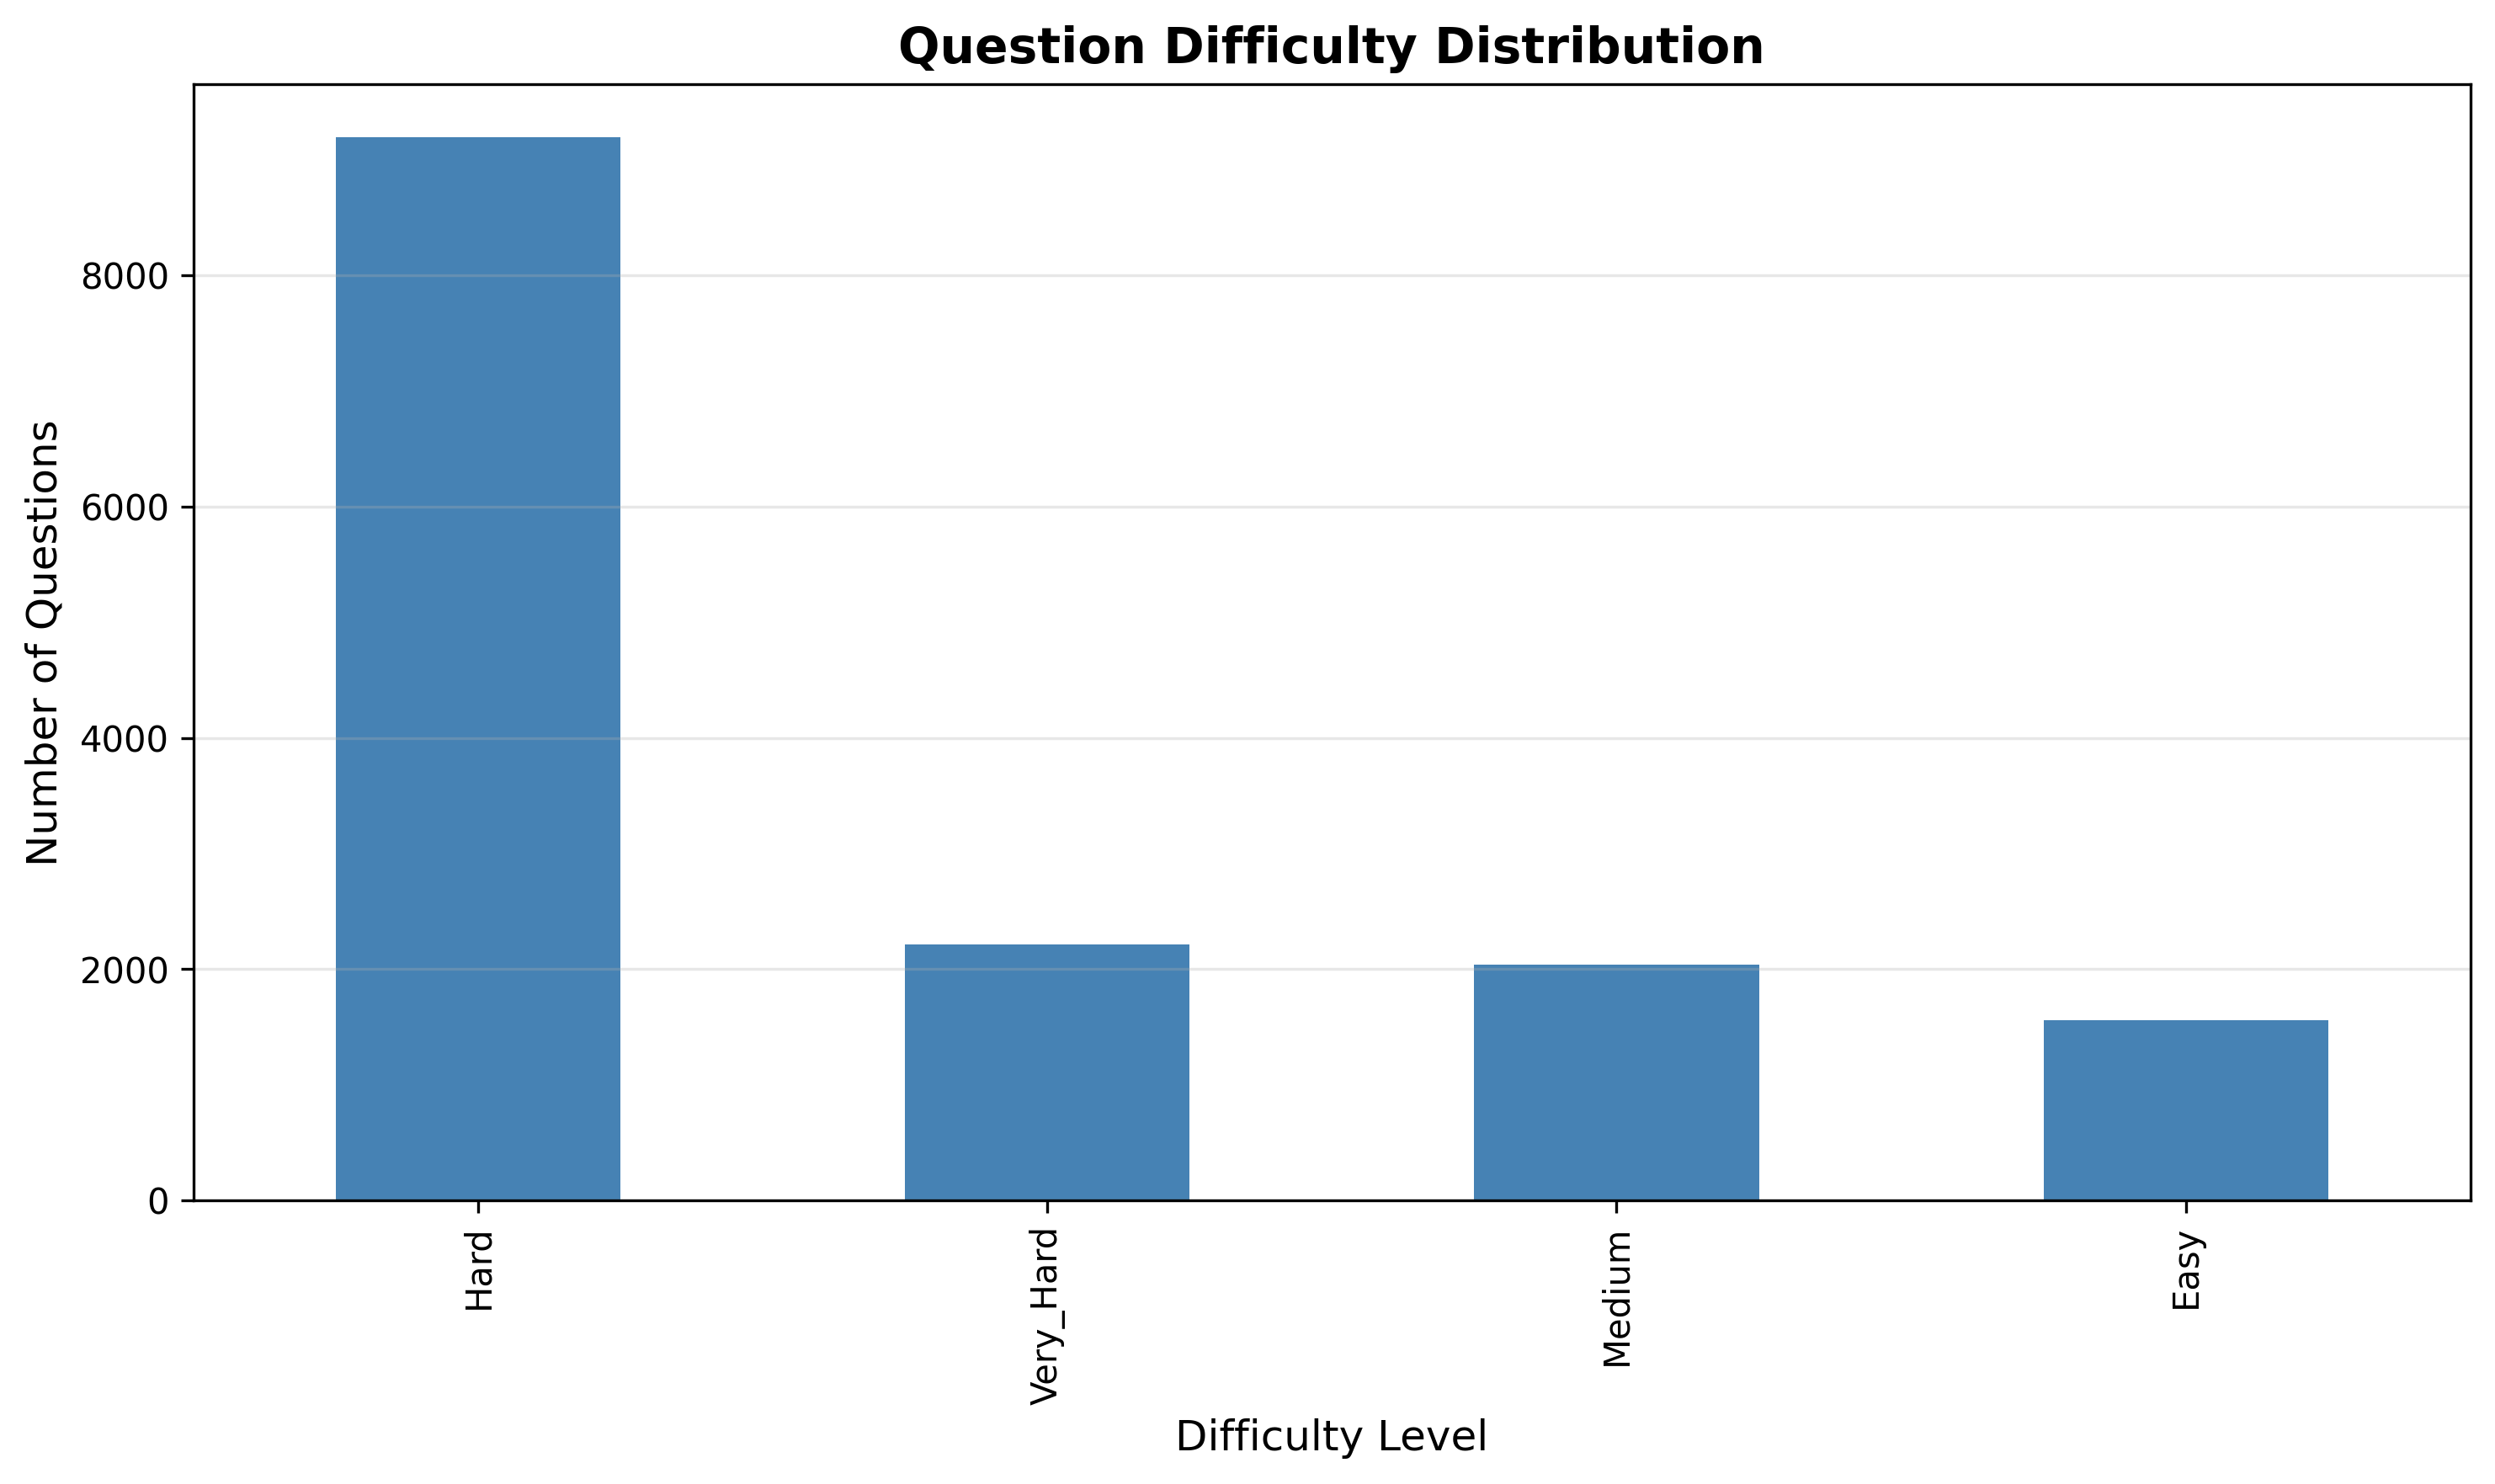
\includegraphics[width=0.8\textwidth]{figures/difficulty_distribution_bar.png}
    \caption{Bar chart showing the distribution of questions across difficulty categories.}
    \label{fig:diff-bar}
\end{figure}

\subsection{Hardest Questions Analysis}
Table~\ref{tab:hardest} presents a sample of the most difficult questions identified by the system (lowest accuracy scores).

\begin{table}[H]
\centering
\caption{Top 5 hardest questions (lowest accuracy proxy score)}
\label{tab:hardest}
\begin{tabular}{clr}
\toprule
\textbf{ID} & \textbf{Title (Truncated)} & \textbf{Score} \\
\midrule
688245 & Is there a better Python bundle for TextMate\ldots & $-17.0$ \\
183042 & How can I use UUIDs in SQLAlchemy?             & $-15.0$ \\
688766 & Getting 401 on Twitter OAuth POST requests     & $-1.5$  \\
284115 & Cross platform hidden file detection            & $-1.0$  \\
336753 & Django FormWizard and Admin application         & $-1.0$  \\
\bottomrule
\end{tabular}
\end{table}

% ══════════════════════════════════════
\section{System Architecture}
\label{sec:architecture}
% ══════════════════════════════════════

The system is organised into modular components:

\begin{table}[H]
\centering
\caption{System modules and their responsibilities}
\label{tab:modules}
\begin{tabular}{lll}
\toprule
\textbf{Module} & \textbf{File} & \textbf{Responsibility} \\
\midrule
Data Reduction    & \texttt{scripts/data\_reduction.py}      & Subsample raw CSVs \\
Feature Eng.      & \texttt{scripts/feature\_engineering.py}  & Compute metrics and labels \\
Model Training    & \texttt{notebooks/model\_training.ipynb}  & Train and evaluate classifier \\
Web Application   & \texttt{app.py}                           & Streamlit UI \\
Visualisations    & \texttt{outputs/*.png}                    & Static plots \\
\bottomrule
\end{tabular}
\end{table}

\subsection{Streamlit Application}
The web interface (\texttt{app.py}) provides:
\begin{enumerate}[noitemsep]
    \item \textbf{CSV Upload:} Users upload \texttt{Questions.csv}, \texttt{Answers.csv}, and \texttt{Tags.csv}.
    \item \textbf{Pipeline Execution:} One-click data reduction, feature engineering, and prediction.
    \item \textbf{Results Display:} Table of true vs.\ predicted difficulty, performance metrics, and charts.
\end{enumerate}

\subsection{Model Persistence}
The trained model and vectoriser are serialised using \texttt{joblib}~\cite{joblib}:
\begin{itemize}[noitemsep]
    \item \texttt{models/model.joblib} --- Logistic Regression classifier (758~KB)
    \item \texttt{models/vectorizer.joblib} --- CountVectorizer (447~KB)
    \item \texttt{models/metrics.txt} --- Classification report
\end{itemize}

% ══════════════════════════════════════
\section{Discussion}
\label{sec:discussion}
% ══════════════════════════════════════

\subsection{Strengths}
\begin{itemize}[noitemsep]
    \item End-to-end pipeline from raw data to interactive predictions.
    \item Modular code design with reusable scripts.
    \item Clear difficulty labelling formula grounded in engagement metrics.
    \item Interactive Streamlit interface enabling non-technical users to explore results.
\end{itemize}

\subsection{Limitations}
\begin{itemize}[noitemsep]
    \item \textbf{Class imbalance:} 75\% of questions are labelled \textit{Hard}, causing the model to be biased towards the majority class. Techniques such as SMOTE, class weighting ($\texttt{class\_weight='balanced'}$ in scikit-learn), or threshold tuning should be explored.
    \item \textbf{Single model:} Only Logistic Regression was trained. Comparing with Decision Trees, Random Forests, or gradient-boosted models would provide a more robust baseline.
    \item \textbf{Vectorisation:} CountVectorizer captures word presence but ignores word importance. TF--IDF weighting would down-weight common terms and improve discriminative power.
    \item \textbf{Proxy data:} Stack Overflow engagement metrics are an imperfect proxy for actual exam difficulty. Future work should incorporate real student response data.
\end{itemize}

% ══════════════════════════════════════
\section{Future Work}
\label{sec:future}
% ══════════════════════════════════════

\begin{enumerate}
    \item \textbf{Milestone~2:} Integrate TF--IDF vectorisation and train multiple models (Decision Tree, Random Forest, SVM) with hyperparameter tuning.
    \item \textbf{Class imbalance handling:} Apply SMOTE or adjust class weights.
    \item \textbf{Advanced NLP:} Experiment with word embeddings (Word2Vec, GloVe) or transformer-based models (BERT) for richer text representations.
    \item \textbf{Real exam data:} Collect and integrate actual student response data for ground-truth difficulty labels.
    \item \textbf{Agentic assessment design:} Use the difficulty predictor as part of an agentic system that automatically generates balanced exam papers.
\end{enumerate}

% ══════════════════════════════════════
\section{Conclusion}
\label{sec:conclusion}
% ══════════════════════════════════════

Milestone~1 of the ExamWise project successfully establishes a working pipeline for question difficulty prediction. Starting from raw Stack Overflow data, the system reduces, processes, and labels 15{,}000 questions using an engagement-based difficulty formula. A Logistic Regression classifier trained on Bag-of-Words features achieves $65.71\%$ accuracy, with strong performance on the majority class but poor recall on minority classes due to data imbalance.

The accompanying Streamlit application provides an accessible interface for uploading data, running the pipeline, and visualising results. While the current baseline has clear limitations---single model, no imbalance correction, simple vectorisation---it provides a solid foundation for the more advanced techniques planned in subsequent milestones.

% ══════════════════════════════════════
% References
% ══════════════════════════════════════

\begin{thebibliography}{9}

\bibitem{lord1980applications}
F.~M. Lord, \textit{Applications of Item Response Theory to Practical Testing Problems}.
Hillsdale, NJ: Lawrence Erlbaum Associates, 1980.

\bibitem{hambleton1991fundamentals}
R.~K. Hambleton, H.~Swaminathan, and H.~J. Rogers, \textit{Fundamentals of Item Response Theory}.
Newbury Park, CA: Sage Publications, 1991.

\bibitem{ha2019automated}
L.~A. Ha, V.~Yaneva, P.~Baldwin, and J.~Mee, ``Automated estimation of item difficulty for multiple-choice tests: An application of word embedding techniques,'' in \textit{Proc.\ 14th Workshop on Innovative Use of NLP for Building Educational Applications}, 2019, pp.~370--382.

\bibitem{anderson2012discovering}
A.~Anderson, D.~Huttenlocher, J.~Kleinberg, and J.~Leskovec, ``Discovering value from community activity on focused question answering sites: A case study of Stack Overflow,'' in \textit{Proc.\ 18th ACM SIGKDD Int.\ Conf.\ Knowledge Discovery and Data Mining}, 2012, pp.~850--858.

\bibitem{stacksample}
Stack Overflow, ``StackSample: 10\% of Stack Overflow Q\&A,'' Kaggle, 2016. [Online]. Available: \url{https://www.kaggle.com/datasets/stackoverflow/stacksample}. [Accessed: Feb.\ 20, 2026].

\bibitem{sklearn}
F.~Pedregosa \textit{et al.}, ``Scikit-learn: Machine learning in Python,'' \textit{J.\ Machine Learning Research}, vol.~12, pp.~2825--2830, 2011.

\bibitem{joblib}
Joblib Development Team, ``Joblib: Running Python functions as pipeline jobs.'' [Online]. Available: \url{https://joblib.readthedocs.io/}. [Accessed: Feb.\ 20, 2026].

\end{thebibliography}

% ══════════════════════════════════════
\newpage
\appendix
\section{Project Structure}
\label{app:structure}

\begin{lstlisting}[language=bash, caption={Repository file structure}]
ExamWise/
  app.py                         # Streamlit application
  requirements.txt               # Python dependencies
  scripts/
    data_reduction.py            # Dataset reduction
    feature_engineering.py       # Feature computation and labelling
  models/
    model.joblib                 # Trained LR classifier
    vectorizer.joblib            # Fitted CountVectorizer
    metrics.txt                  # Classification report
  notebooks/
    model_training.ipynb         # Training notebook
  outputs/
    difficulty_distribution.png  # Difficulty bar chart
    accuracy_distribution.png    # Accuracy histogram
    hardest_questions.csv        # Hardest questions table
  docs/
    MODEL_CARD.md                # Model documentation
    problem_statement.md         # Problem definition
    system_architecture.md       # Architecture overview
  report/
    main.tex                     # This report (LaTeX)
    references.bib               # Bibliography
    figures/                     # Report figures
\end{lstlisting}

\section{Team Contributions}
\label{app:contributions}

\begin{table}[H]
\centering
\caption{Role-wise work allocation for Milestone~1}
\begin{tabular}{lp{8cm}}
\toprule
\textbf{Role} & \textbf{Contributions} \\
\midrule
Person~1 (Data \& Labelling) & Dataset acquisition, data reduction script, feature engineering, difficulty labelling, processed CSV export \\
Person~2 (Features \& Models) & Model training, CountVectorizer pipeline, Logistic Regression classifier, evaluation metrics, model serialisation \\
Person~3 (Analytics \& Visualisations) & Difficulty distribution charts, accuracy analysis, hardest questions identification, output generation \\
Person~4 (App \& Integration) & Streamlit application, README documentation, requirements specification, Git management \\
\bottomrule
\end{tabular}
\end{table}

\end{document}
